% Created 2016-06-01 mer. 15:49
\documentclass[smaller]{beamer}
\usepackage[utf8]{inputenc}
\usepackage[T1]{fontenc}
\usepackage{fixltx2e}
\usepackage{graphicx}
\usepackage{longtable}
\usepackage{float}
\usepackage{wrapfig}
\usepackage{rotating}
\usepackage[normalem]{ulem}
\usepackage{amsmath}
\usepackage{textcomp}
\usepackage{marvosym}
\usepackage{wasysym}
\usepackage{amssymb}
\usepackage{hyperref}
\tolerance=1000
\usepackage[T1]{fontenc}
\usepackage[english, french]{babel}
\useoutertheme{infolines}
\mode<beamer>{\usetheme{Pittsburgh}}
\setbeamertemplate{navigation symbols}{}
\setbeamerfont{structure}{series=\bfseries}
\setbeamertemplate{items}[triangle]
\setbeamercolor{block title}{fg=blue!40!black}
\newcommand{\shorttitle}{OTB User Days, June 7-9 2016}
\newcommand{\shortauthor}{}
\setbeamertemplate{footline}{\leavevmode\hbox{\begin{beamercolorbox}[wd=.333333\paperwidth,ht=2.25ex,dp=1ex,left]{author in head/foot}  \usebeamerfont{author in headfoot}\insertshortinstitute~~\shortauthor   \end{beamercolorbox}   \begin{beamercolorbox}[wd=.333333\paperwidth,ht=2.25ex,dp=1ex,center]{title   in head/foot}     \usebeamerfont{title in head/foot}\shorttitle   \end{beamercolorbox}   \begin{beamercolorbox}[wd=.333333\paperwidth,ht=2.25ex,dp=1ex,right]{date in head/foot}\usebeamerfont{date in head/foot}\insertshortdate{} \hspace*{2em}\insertframenumber{} / \inserttotalframenumber\hspace*{2ex} \end{beamercolorbox}}\vskip0pt}
\institute{ 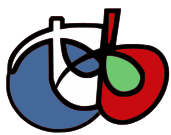
\includegraphics[width=0.6cm]{images/logoIncrust.png}}
\usepackage{fourier}
\usepackage{amsfonts,bm,amsmath,amssymb,ifsym,marvosym,tabularx,array,ifsym}
\usepackage{tikz}
\usetikzlibrary{arrows,fit,backgrounds,positioning,shapes,shadows}
\newcommand{\vns}{Ven$\mu$s}
\newcommand\boxPlot[6] {  \pgfmathsetmacro\rectSize{0.3};  \draw[thick] (#2,#1) -- (#3,#1);  \draw[thick] (#2,#1-\rectSize/2) -- (#2,#1+\rectSize/2);  \draw[thick] (#5,#1) -- (#6,#1);  \draw[thick] (#6,#1-\rectSize/2) -- (#6,#1+\rectSize/2);  \draw[fill=white] (#3,#1-\rectSize) rectangle (#5,#1+\rectSize);  \draw (#4,#1-\rectSize) -- (#4,#1+\rectSize);}
\def\G{\ensuremath{{\cal G}}}
\newcommand{\putat}[3]{\begin{picture}(0,0)(0,0)\put(#1,#2){#3}\end{picture}}
\pgfdeclareimage[height=96mm,width=130mm]{background}{images/fondsClairSansLogo}
\setbeamertemplate{background}{\pgfuseimage{background}}
\usetheme{default}
\author{OTB Team}
\date{07/06/2016}
\title{Monteverdi Whats New}
\hypersetup{
  pdfkeywords={otb},
  pdfsubject={},
  pdfcreator={Emacs 24.3.1 (Org mode 8.2.4)}}
\begin{document}

\maketitle
% Emacs 24.3.1 (Org mode 8.2.4)

\section{Introduction}
 
\begin{frame}{One year since the HackFest}

Last year, we decide together the roadmap of Monteverdi.

Major changes during this year:
\begin{itemize}
  \item Database/Respository and persistent settings abandoned
  \item Monteverdi is (now) a lightweight Viewer
  \item Switch from Monteverdi2 v-0.8 to \textbf{Monteverdi v-3.2.0}
\end{itemize}

\end{frame}

\begin{frame}{A second user tool for OTB}

MAPLA (Monteverdi APplication LAuncher)
\begin{itemize}
  \item WYSIWYG GUI
  \item OTB-applications browser (grouped by tag)
  \item Interactive search bar
  \item Double-click to show GUI of OTB-application (multi-instance)
  \item File system explorer filename drag-n-drop
\end{itemize}

\begin{figure}[ht]
\begin{center}
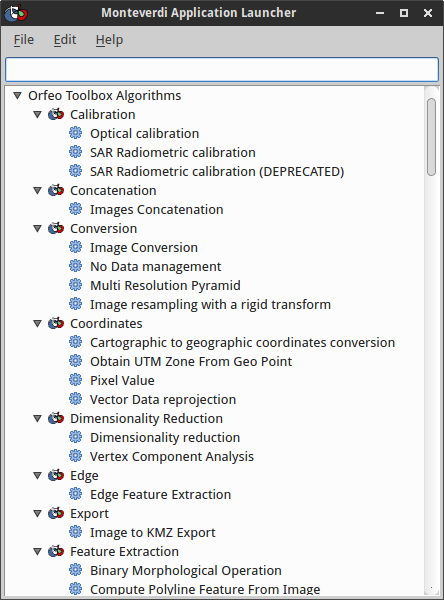
\includegraphics[scale=0.23]{images/2016-06-06_MVD_Mapla.png}
\end{center}
\end{figure}

\end{frame}

\section{New Features}

\begin{frame}{Multi Image-Layer Mode}

\begin{figure}[ht]
\begin{center}
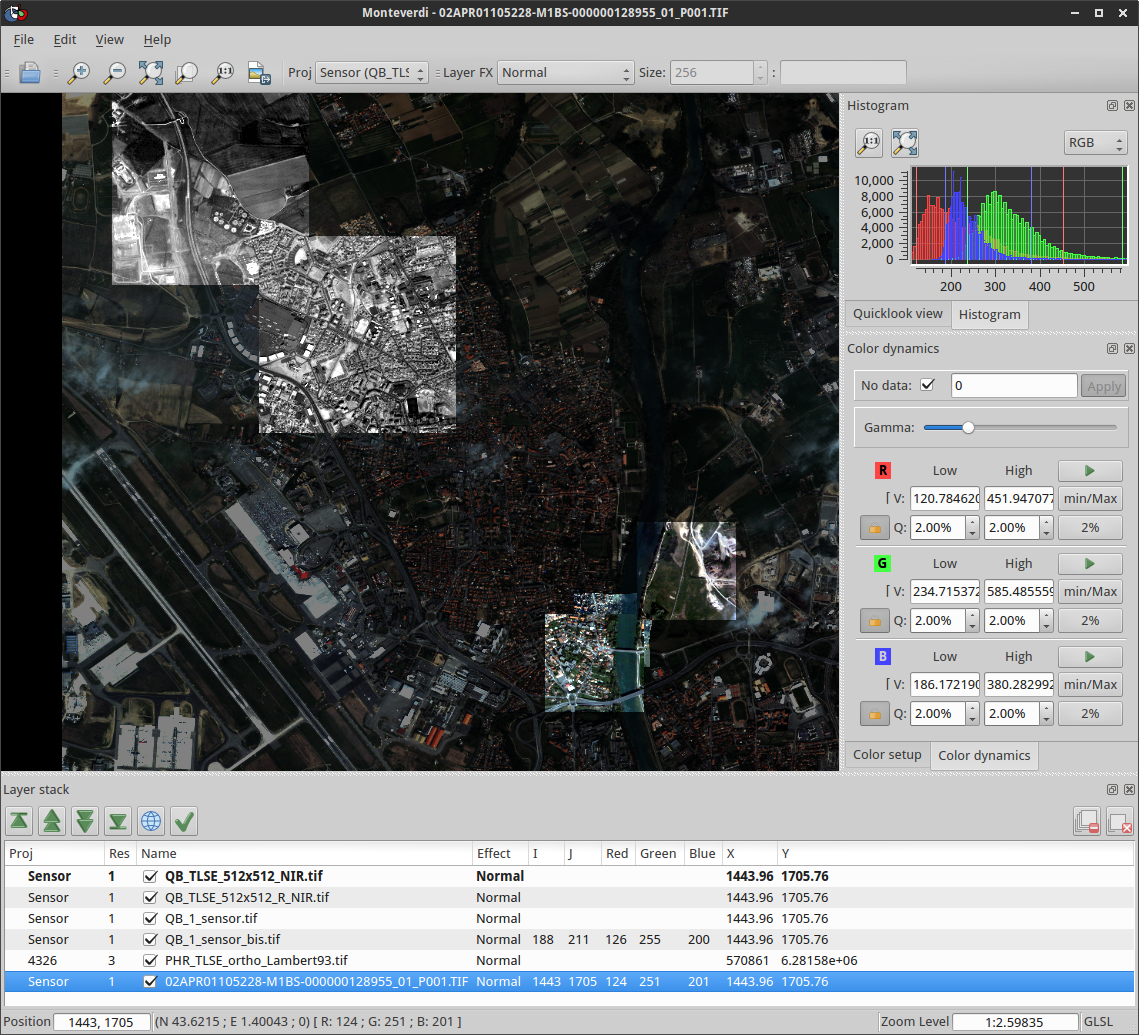
\includegraphics[height=2.1in]{images/2016-06-06_MVD_Multi_Image-Layer_Support.png}
\end{center}
\end{figure}

\begin{itemize}
  \item Geo-referenced display of several images (heterogeneous)
  \item OTB-Ice rendering engine
  \item Many performance bugfixes/optimizations
  \item Choose reference projection system
  \item On-the-fly reprojection of images into reference system
\end{itemize}

\end{frame}

\begin{frame}{Layer management}

\begin{figure}[ht]
\begin{center}
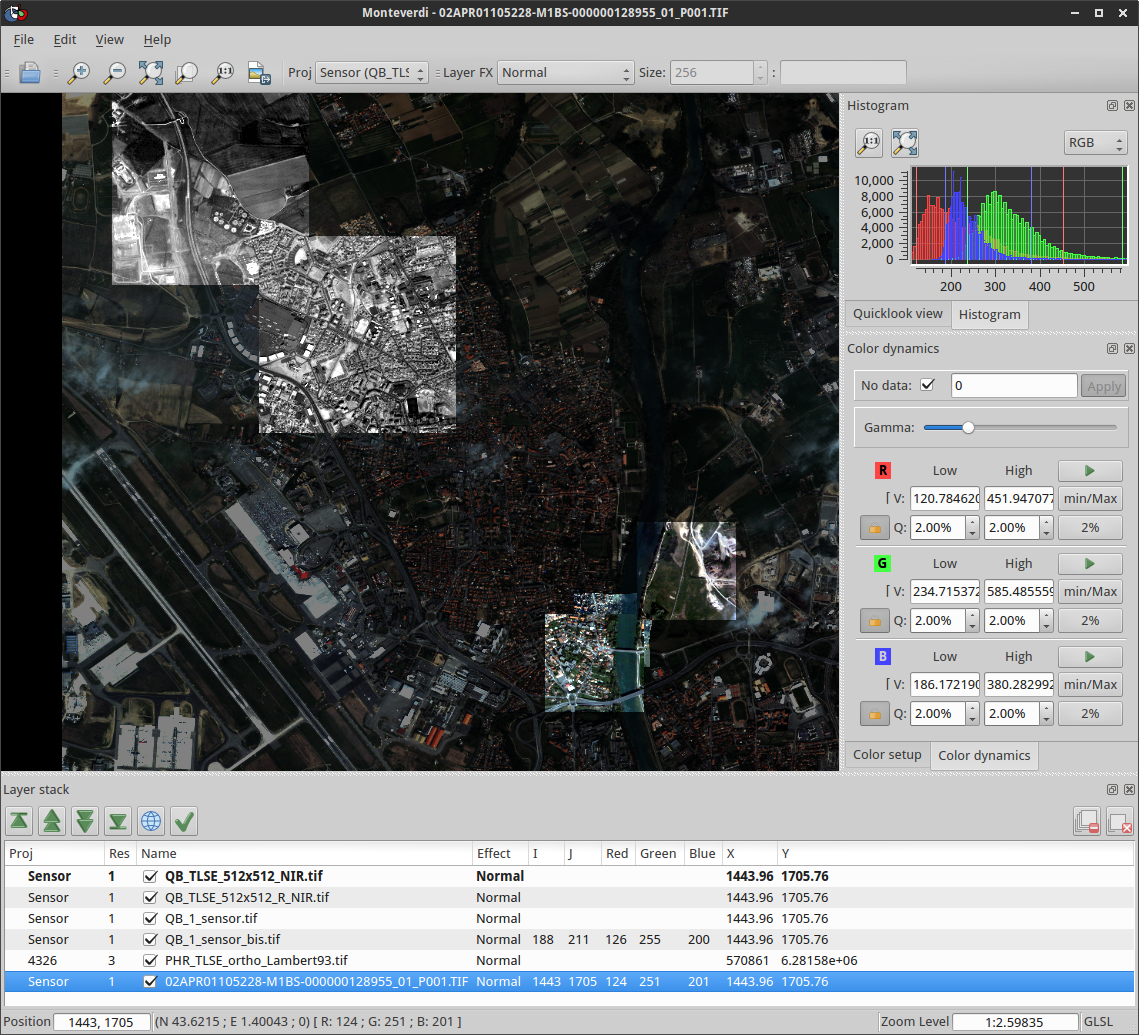
\includegraphics[height=2.1in]{images/2016-06-06_MVD_Multi_Image-Layer_Support.png}
\end{center}
\end{figure}

\begin{itemize}
  \item Edit order of superposition
  \item Set reference projection system
  \item Image information display: projection system, displayed resolution, effect etc.
  \item Pixel information display: index, position, RGB intensities
\end{itemize}

\end{frame}

\begin{frame}{Visualization Tools/Effects}

\begin{figure}[ht]
\begin{center}
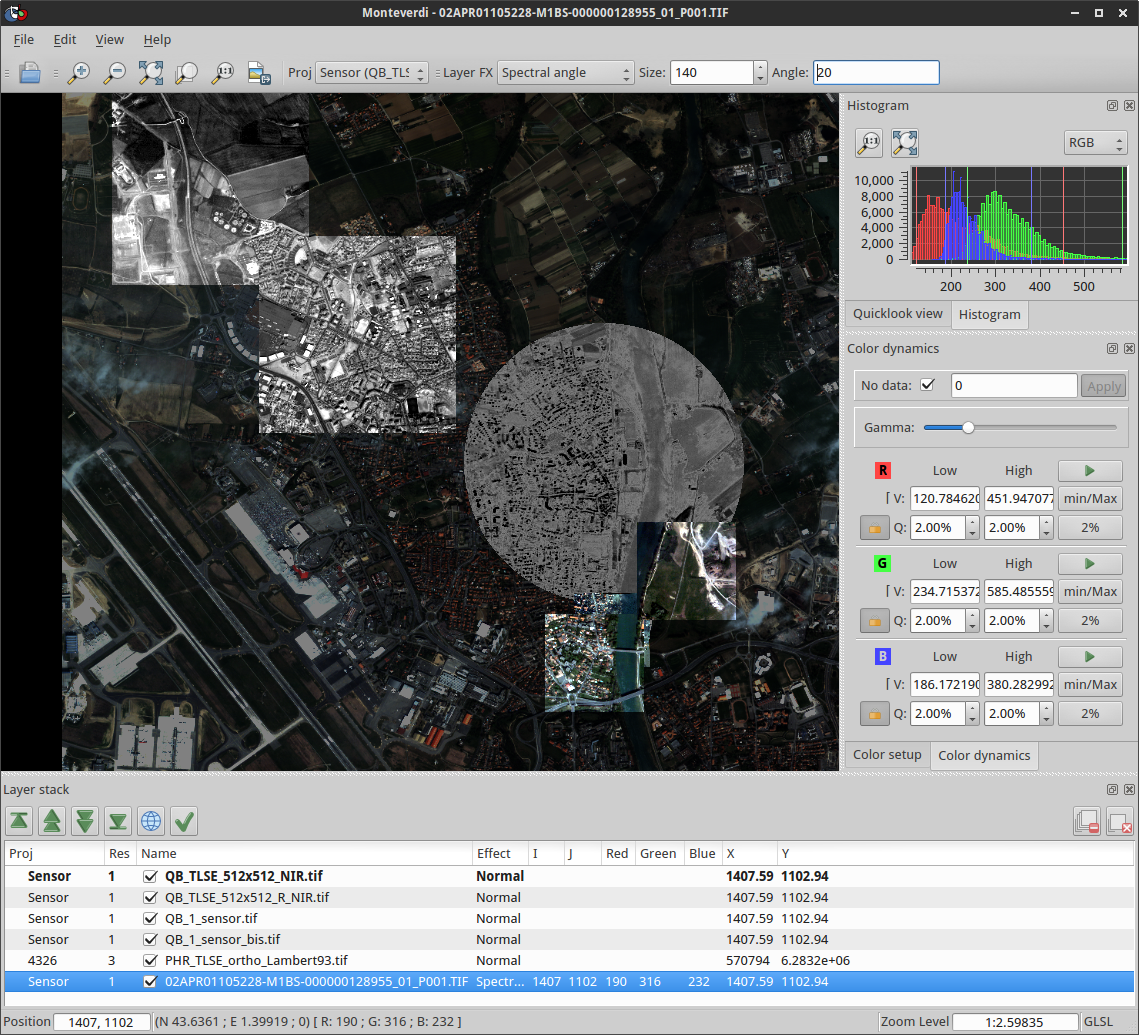
\includegraphics[height=2.1in]{images/2016-06-06_MVD_Multi_Image-Layer_Support_2.png}
\end{center}
\end{figure}

\begin{itemize}
  \item Local contrast, Spectral Angle, Gradient etc. (by layer)
  \item Zooming: full extent, layer extent and 1:1 scale
  \item Numerous keyboard/mouse shortcuts of GUI controls (interactivity)
  \item Screenshot facility
  \item Rendering preferences
\end{itemize}

\end{frame}

\begin{frame}{Improve OTB-application integration}

\begin{figure}[ht]
\begin{center}
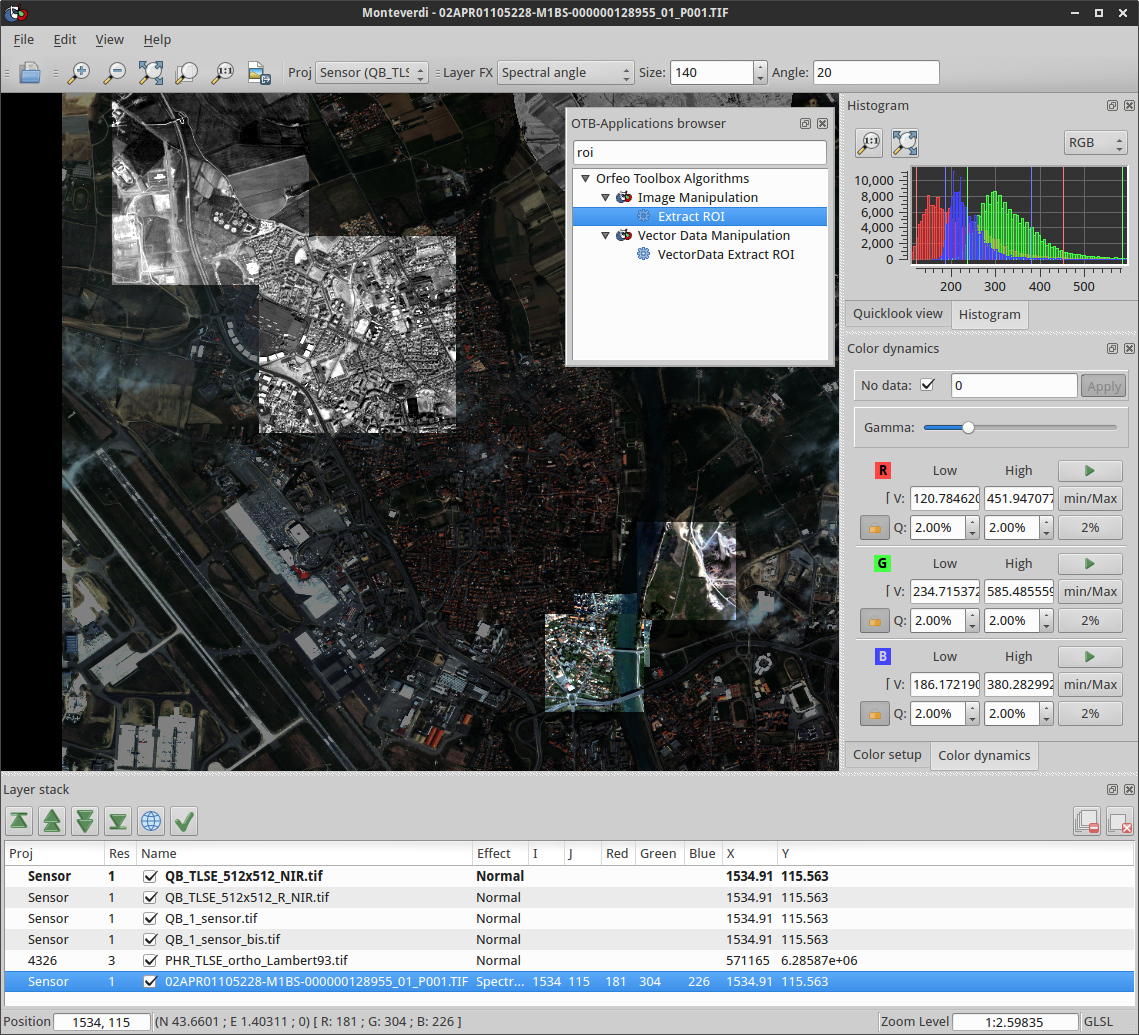
\includegraphics[height=2.1in]{images/2016-06-06_MVD_OTB-applications.png}
\end{center}
\end{figure}

\begin{itemize}
  \item On-Demand loading (via File menu): Saves startup time when using viewer-mode only
  \item Same features as Mapla AND Dockable panel AND Layer drag-n-drop 
\end{itemize}

\end{frame}

\begin{frame}{Image Import with multiple files selection}

\begin{itemize}
  \item File/Open... popup with multi-selection
  \item Command line to pass several files 
\end{itemize}

\end{frame} 
   
\begin{frame}{Multi-Resolution Pyramid Configuration (GDAL overviews)}   

\begin{figure}[ht]
\begin{center}
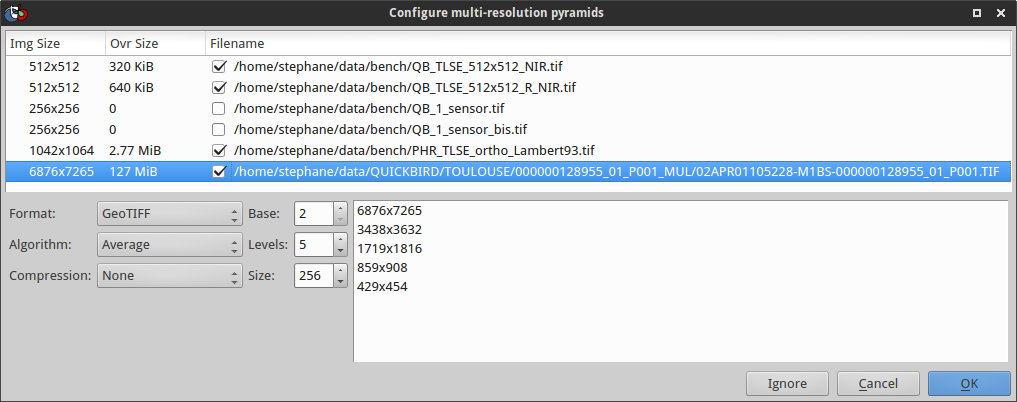
\includegraphics[height=1.5in]{images/2016-06-06_MVD_Multi-Resolution_Pyramid_configuration.png}
\end{center}
\end{figure}

\begin{itemize}
  \item Multiple-selection list of files
  \item Image information: size, real/estimated disk space
  \item By image setup: default configuration or set decimation factors, format, algorithm, compression
  \item Size of multi-resolution pyramid levels
\end{itemize}   

\end{frame}    
   
\begin{frame}{Compound Dataset Support (CDS)}      

\begin{figure}[ht]
\begin{center}
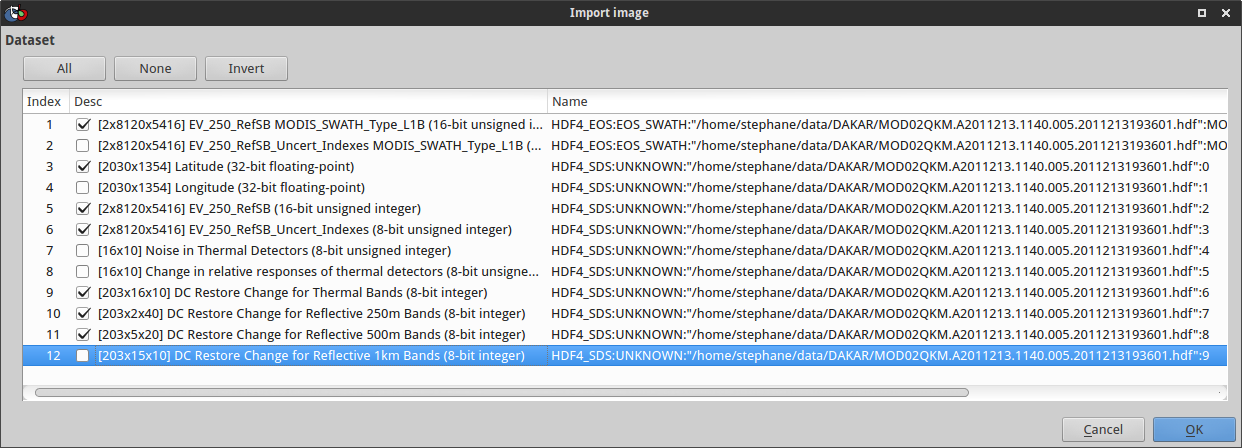
\includegraphics[height=1.5in]{images/2016-06-06_MVD_Compound_Dataset_Support.png}
\end{center}
\end{figure}

\begin{itemize}
   \item Multiple-selection list
   \item Sub-dataset info (index, name, description)
   \item Useful for Sentinel-2 data
\end{itemize}

\end{frame} 

\begin{frame}{Remote Desktop-Mode}   
\textit{Problematic}:
\begin{itemize}  
   \item OTB-Ice required OpenGL 2.x and OpenGL Shading Language (GLSL) 1.20
   \item Not supported by all users platforms and Remote-Desktop Protocols
   \item Monteverdi was locked if OpenGL/GLSL requirements were not met
   \item Many people use OTB via Remote-Desktop Protocols or low graphics platforms
\end{itemize} 

\textit{Solution}:
\begin{itemize}  
   \item Implemented OpenGL 1.x compatibility mode:
   \begin{itemize} 
     \item OpenGL textures and ITK iterators used for multi-image rendering
     \item Layer effects disabled
   \end{itemize}   
   \item Add OpenGL/GLSL tag in status-bar (lower-right corner)
   \item  Pros:
   \begin{itemize} 
     \item Monteverdi now runs on more systems
     \item Monteverdi access is eased to more people
   \end{itemize}  
   \item Cons:
   \begin{itemize} 
     \item Rendering performances are lowered (compared to GLSL rendering)
     \item Layer effects are disabled
   \end{itemize} 
\end{itemize} 

\end{frame} 

\section{Conclusion}

\begin{frame}{Next Steps?}
\textbf{2015 goals have been fulfilled :)}


Overall topics:
\begin{itemize}   
  \item User keymap documentation (Help/Keymap...)
  \item GUI layout saved/restored
\end{itemize} 


Goodies: Monteverdi and Mapla binaries comes in OTB standalone binary packages 

Coming soon: Merge source-code repositories (OTB and Monteverdi)

\textbf{Roadmap?}
\begin{itemize}
   \item Interactive ROI editing
   \item Save layer-stack as XML project
   \item SAR complex-data images display
   \item Spectral profile tools
   \item Vector-Data
   \item Feedback are welcome !
\end{itemize}

\end{frame} 

\end{document}
